\documentclass[a4paper,12pt]{article}
\usepackage{settings} % Подгружает наш исправленный settings.sty

\begin{document}

% ==================== ТИТУЛЬНЫЙ ЛИСТ ====================
\thispagestyle{empty}

\begin{table}[h!]
\centering
\begin{tabular}{p{0.65\textwidth}r}
    \begin{tabular}{@{}l}
        \footnotesize{Университет ИТМО} \\
        \footnotesize{Физико-технический мегафакультет} \\
        \footnotesize{Физический факультет}
    \end{tabular} & 
    \raisebox{-0.5\height}{
\includegraphics[width=0.22\linewidth]{logo_ITMO.pdf}}
\end{tabular}
\end{table}

\vspace{0.5cm}

\begin{center}
\begin{tabular}{p{0.49\textwidth}p{0.49\textwidth}}
Группа \textbf{K3242} & К работе допущен \hrulefill \\
& \\
Студент \textbf{Шумилов А. К.} & Работа выполнена \hrulefill \\
& \\
Преподаватель \textbf{Курашова С. А.} & Отчет принят \hrulefill \\
\end{tabular}
\end{center}

\vspace{1.5cm}

\begin{center}
    \large{\textbf{Рабочий протокол и отчет по\\лабораторной работе № 3.03}} \\
    \vspace{0.8cm}
    \large{\textbf{«Определение удельного заряда электрона методом магнетрона»}}
\end{center}

\newpage
\setcounter{page}{2}
\pagestyle{plain}

% ==================== ОСНОВНОЙ ТЕКСТ ====================

\section*{\hspace{30pt}1. Цель работы}
\hspace{15pt} Экспериментальное определение удельного заряда электрона $e/m$ методом магнетрона, исследование движения электронов в скрещенных электрическом и магнитном полях в вакуумном диоде цилиндрической геометрии.

\section*{\hspace{30pt}2. Задачи, решаемые при выполнении работы}
\begin{enumerate}
    \setlength{\itemindent}{15pt}
    \item Провести измерения зависимости анодного тока $I_a$ вакуумного диода от тока соленоида $I_L$ при анодных напряжениях $8, 10, 12, 14$ и $15$~В.
    \item Построить графики зависимостей анодного тока $I_a$ от тока соленоида $I_L$, а также графики их производных для каждого значения анодного напряжения.
    \item Определить критические значения тока соленоида $I_{L\text{кр}}$ и соответствующие им критические магнитные индукции $B_c$.
    \item Вычислить удельный заряд электрона $e/m$ по формуле метода магнетрона для каждого анодного напряжения, найти среднее значение и оценить погрешность.
    \item Построить график зависимости $B_c^2$ от анодного напряжения $U$ и определить $e/m$ из углового коэффициента полученной прямой методом наименьших квадратов (МНК).
\end{enumerate}

\section*{\hspace{30pt}3. Объект исследования}
\hspace{15pt} Вакуумный коаксиально-цилиндрический диод с малым радиусом катода, помещенный внутрь соленоида, создающего однородное продольное магнитное поле.

\section*{\hspace{30pt}4. Метод экспериментального исследования}
\hspace{15pt} Метод основан на закручивании траекторий электронов силой Лоренца в скрещенных полях. При достижении критической индукции $B_c$ траектории становятся касательными к аноду, вызывая резкое падение анодного тока. При высоких напряжениях ($14$ и $15$~В) метод дополняется фиксацией пика вторичной электронной эмиссии при возвращении электронов на катод, причем критический ток фиксируется строго перед началом этого пика.

\section*{\hspace{30pt}5. Схема экспериментальной установки}
\begin{figure}[H]
    \centering
    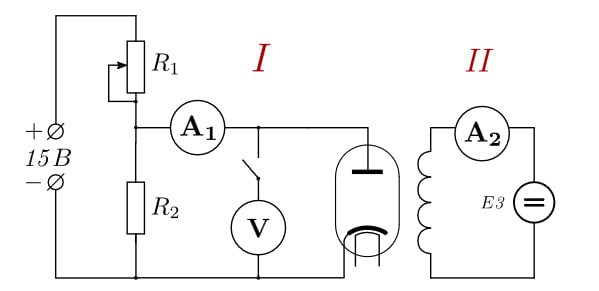
\includegraphics[width=0.7\textwidth]{shema_ustanovki.png} 
    \caption{Принципиальная электрическая схема измерительного стенда для метода магнетрона}
    \label{fig:setup}
\end{figure}

\section*{\hspace{30pt}6. Рабочие формулы и исходные данные}
\hspace{15pt} Магнитная индукция в центре соленоида конечной длины рассчитывается по формуле:
\begin{equation}
    B_{c} = \frac{\mu_{0} \cdot N \cdot I_{L\text{кр}}}{\sqrt{l^{2} + d^{2}}},
    \label{eq:b_field}
\end{equation}
where $\mu_{0} = 4\pi \cdot 10^{-7}$~Гн/м; число витков соленоида $N = 1500$; геометрические параметры соленоида установки ИТМО: длина $l = 0.036$~м, диаметр $d = 0.037$~м.

Расчетная формула удельного заряда электрона (с учетом геометрии коаксиального диода, где радиус катода $R_k \ll R_a$):
\begin{equation}
    \frac{e}{m} = \frac{8U}{(B_c \cdot R_a)^2} = \frac{8U(l^2 + d^2)}{(\mu_0 \cdot R_a \cdot N \cdot I_{L\text{кр}})^2},
    \label{eq:edm}
\end{equation}
where $R_a = 0.003$~м — радиус анода диода.

\section*{\hspace{30pt}7. Измерительные приборы}
\hspace{15pt} В соответствии с методическими указаниями и поправками к стенду, измерительные приборы имеют следующие характеристики:
\begin{table}[H]
    \caption{Характеристики измерительных приборов стенда}
    \label{tab:devices}
    \centering
    \begin{tabular}{|c|c|c|c|c|}
        \hline
        № & Наименование & Тип & Режим / Диапазон & Погрешность \\ \hline
        1 & Амперметр анодного тока & MY64 & Пост. ток, 2~мА & $\pm(0.5\% + 1~\text{ед.})$ \\ \hline
        2 & Амперметр тока соленоида & MY65 & Пост. ток, 2~А / 20~А & $\pm(0.5\% + 1~\text{ед.})$ \\ \hline
        3 & Вольтметр анодный & Встроенный & Пост. напряжение, 0--15~В & $\pm 1.0\%$ \\ \hline
    \end{tabular}
\end{table}

\section*{\hspace{30pt}8. Результаты прямых измерений}
\hspace{15pt} Ниже представлены твои экспериментальные зависимости анодного тока $I_a$ (мА) от тока соленоида $I_L$ (А):
\begin{longtable}{|c|c|c|c|c|c|}
    \caption{Экспериментальные зависимости анодного тока от тока катушки} \label{tab:raw_data} \\
    \hline
    $I_L$, А & $U = 8$~В & $U = 10$~В & $U = 12$~В & $U = 14$~В & $U = 15$~В \\ \hline
    0.00 & 0.1751 & 0.2332 & 0.2916 & 0.3561 & 0.3861 \\ \hline
    0.02 & 0.1760 & 0.2334 & 0.2912 & 0.3558 & 0.3853 \\ \hline
    0.04 & 0.1762 & 0.2332 & 0.2913 & 0.3562 & 0.3854 \\ \hline
    0.06 & 0.1763 & 0.2337 & 0.2913 & 0.3560 & 0.3850 \\ \hline
    0.08 & 0.1758 & 0.2354 & 0.2927 & 0.3563 & 0.3851 \\ \hline
    0.10 & 0.1762 & 0.2333 & 0.2929 & 0.3569 & 0.3858 \\ \hline
    0.12 & 0.1764 & 0.2336 & 0.2927 & 0.3564 & 0.3865 \\ \hline
    0.14 & 0.1752 & 0.2339 & 0.2932 & 0.3570 & 0.3880 \\ \hline
    0.16 & 0.1750 & 0.2338 & 0.2936 & 0.3582 & 0.3889 \\ \hline
    0.18 & 0.1732 & 0.2320 & 0.2926 & 0.3579 & 0.3889 \\ \hline
    0.20 & 0.1689 & 0.2280 & 0.2892 & 0.3544 & 0.3860 \\ \hline
    0.22 & 0.1573 & 0.2140 & 0.2810 & 0.3463 & 0.3793 \\ \hline
    0.24 & 0.1164 & 0.1740 & 0.2403 & 0.3237 & 0.3645 \\ \hline
    0.26 & 0.0994 & 0.1367 & 0.1972 & 0.2525 & 0.2839 \\ \hline
    0.28 & 0.0797 & 0.1131 & 0.1596 & 0.1988 & 0.2250 \\ \hline
    0.30 & 0.0708 & 0.1035 & 0.1348 & 0.1720 & 0.1850 \\ \hline
    0.32 & 0.0613 & 0.0924 & 0.1232 & 0.1572 & 0.1724 \\ \hline
    0.34 & 0.0512 & 0.0797 & 0.1122 & 0.1477 & 0.1610 \\ \hline
    0.36 & 0.0469 & 0.0727 & 0.0977 & 0.1336 & 0.1450 \\ \hline
    0.38 & 0.0402 & 0.0644 & 0.0900 & 0.1167 & 0.1333 \\ \hline
    0.40 & 0.0365 & 0.0574 & 0.0816 & 0.1073 & 0.1207 \\ \hline
    0.42 & 0.0334 & 0.0518 & 0.0745 & 0.0985 & 0.1102 \\ \hline
    0.44 & 0.0305 & 0.0477 & 0.0683 & 0.0896 & 0.1011 \\ \hline
    0.46 & 0.0282 & 0.0432 & 0.0617 & 0.0825 & 0.0927 \\ \hline
    0.48 & 0.0261 & 0.0404 & 0.0570 & 0.0762 & 0.0870 \\ \hline
    0.50 & 0.0244 & 0.0380 & 0.0530 & 0.0702 & 0.0790 \\ \hline
    0.52 & 0.0230 & 0.0353 & 0.0496 & 0.0668 & 0.0751 \\ \hline
    0.54 & 0.0219 & 0.0334 & 0.0474 & 0.0634 & 0.0696 \\ \hline
    0.56 & 0.0208 & 0.0320 & 0.0442 & 0.0598 & 0.0667 \\ \hline
    0.58 & 0.0199 & 0.0302 & 0.0422 & 0.0565 & 0.0639 \\ \hline
    0.60 & 0.0188 & 0.0291 & 0.0405 & 0.0540 & 0.0608 \\ \hline
    0.62 & 0.0180 & - & 0.0387 & 0.0516 & 0.0575 \\ \hline
\end{longtable}

\section*{\hspace{30pt}9. Результаты косвенных измерений и их обработки (таблицы, примеры расчетов)}

\subsection*{9.1. Графическое определение критических токов соленоида геометрическим способом}
Определение критического тока $I_{L\text{кр}}$ проводилось геометрическим методом путем аппроксимации пологих участков графика прямыми линиями. Искомое значение фиксировалось в точке пересечения экспериментальной кривой со срединной линией, проведенной ровно посередине между этими прямыми.

\subsection*{9.2. Расчет параметров критического режима и удельного заряда электрона}

\begin{table}[H]
    \caption{Результаты расчетов параметров критического режима и удельного заряда электрона}
    \label{tab:results_calc_full}
    \centering
    \begin{tabular}{|c|c|c|c|c|c|c|c|}
        \hline
        $U$, & $I_{L\text{кр}}$, & $B_c$, & $\varepsilon_B$, & $\Delta B_c$, & $e/m$, & $\Delta(e/m)$, & $\varepsilon_{e/m}$, \\ 
        В & А & Тл & \% & Тл & $10^{11}$ Кл/кг & $10^{11}$ Кл/кг & \% \\ \hline
        8.0  & 0.240 & 0.00876 & 0.8 & 0.00007 & 0.926 & 0.018 & 1.9 \\ \hline
        10.0 & 0.248 & 0.00906 & 0.8 & 0.00007 & 1.084 & 0.020 & 1.8 \\ \hline
        12.0 & 0.252 & 0.00920 & 0.8 & 0.00007 & 1.260 & 0.021 & 1.7 \\ \hline
        14.0 & 0.260 & 0.00949 & 0.8 & 0.00007 & 1.381 & 0.023 & 1.6 \\ \hline
        15.0 & 0.270 & 0.00986 & 0.7 & 0.00007 & 1.372 & 0.022 & 1.6 \\ \hline
    \end{tabular}
\end{table}

\textit{Пример вычислений для первой строки:}
\begin{gather*}
    B_c = \frac{\mu_0 \cdot N}{\sqrt{l^2 + d^2}} \cdot I_{L\text{кр}} = \frac{1.25664 \cdot 10^{-6} \cdot 1500}{\sqrt{0.036^2 + 0.037^2}} \cdot 0.240 \approx 0.00876 \text{ Тл} \\
    \frac{e}{m} = \frac{8U}{B_c^2 \cdot R_a^2} = \frac{8 \cdot 8.0}{(0.00876)^2 \cdot (0.003)^2} \approx 0.926 \cdot 10^{11} \text{ Кл/кг} \\
    \varepsilon_B = \frac{\Delta I_L}{I_{L\text{кр}}} = \frac{0.002}{0.240} \approx 0.0083 \\
    \varepsilon_{e/m} = \sqrt{\left(\frac{\Delta U}{U}\right)^2 + (2 \cdot \varepsilon_B)^2} = \sqrt{\left(\frac{0.08}{8.0}\right)^2 + (2 \cdot 0.0083)^2} \approx 0.019 \\
    \Delta(e/m) = \frac{e}{m} \cdot \varepsilon_{e/m} = 0.926 \cdot 10^{11} \cdot 0.019 \approx 0.018 \cdot 10^{11} \text{ Кл/кг} \\
    \frac{e}{m} = (0.926 \pm 0.018) \cdot 10^{11} \text{ Кл/кг}
\end{gather*}

\subsection*{9.3. Расчет производной $\Delta I_a / \Delta I_L$}
Для уточнения результатов был применен метод численного дифференцирования, основанный на поиске максимума скорости падения анодного тока. Из исходного массива данных были отобраны индивидуальные участки с наибольшей крутизной наклона, что позволило исключить влияние инструментальных шумов на участках плато. Критический ток определялся по положению максимума производной, соответствующего точке наиболее интенсивного магнитного отсечения электронов.

\subsection*{9.4. Рассмотрение удельных зарядов как результаты многократных измерений}
Используем точные значения удельных зарядов из таблицы (приведя их к одному порядку $10^{11}$): 
0.926; 1.084; 1.260; 1.381; 1.372;
\begin{gather*}
    \langle e/m \rangle = \frac{\sum (e/m)_i}{5} \approx 1.205 \cdot 10^{11} \text{ Кл/кг} \\
    S \approx 0.196 \cdot 10^{11} \text{ Кл/кг} \\
    \text{Для } (P = 0.95, t = 2.78) \\
    \Delta(e/m)_{\text{случ}} = 2.78 \cdot \frac{0.196}{\sqrt{5}} \approx 0.244 \cdot 10^{11} \text{ Кл/кг} \\
    e/m = (1.20 \pm 0.24) \cdot 10^{11} \text{ Кл/кг}
\end{gather*}

\subsection*{9.5. Расчет углового коэффициента прямой $B_c^2(U)$ методом наименьших квадратов}
\begin{table}[H]
    \centering
    \begin{tabular}{|c|c|c|c|c|}
        \hline
        $i$ & $x_i$ ($U$, В) & $y_i$ ($B_c^2 \cdot 10^{-6}$) & $x_i y_i$ & $x_i^2$ \\ \hline
        1 & 8.0  & 76.79 & 614.32  & 64.0  \\ \hline
        2 & 10.0 & 81.99 & 819.90  & 100.0 \\ \hline
        3 & 12.0 & 84.66 & 1015.92 & 144.0 \\ \hline
        4 & 14.0 & 90.12 & 1261.68 & 196.0 \\ \hline
        5 & 15.0 & 97.20 & 1458.00 & 225.0 \\ \hline
        $\sum_i$ & 59.0 & 430.76 & 5169.82 & 729.0 \\ \hline
    \end{tabular}
\end{table}

\begin{gather*}
    k = \frac{\sum U_i \cdot B_{c, i}^2}{\sum U_i^2} = \frac{5169.82}{729.0} \approx 7.092 \cdot 10^{-6} \text{ Тл}^2\text{/В} \\
    \sum (B_{c, i}^2 - k U_i)^2 = 693.29 \\
    S_{B^2}^2 = \frac{693.29}{5 - 2} \approx 231.1 \\
    \Delta k = 2.78 \cdot \sqrt{\frac{231.1}{729.0}} \approx 1.56 \cdot 10^{-6} \text{ Тл}^2\text{/В} \\
    \frac{e}{m} = \frac{8}{k \cdot R_a^2} = \frac{8}{7.092 \cdot 10^{-6} \cdot (0.003)^2} \approx 1.253 \cdot 10^{11} \text{ Кл/кг} \\
    \varepsilon = \frac{\Delta k}{k} = \frac{1.56}{7.092} \approx 0.22 \\
    \Delta(e/m) = 1.253 \cdot 10^{11} \cdot 0.22 \approx 0.28 \cdot 10^{11} \text{ Кл/кг} \\
    e/m = (1.25 \pm 0.28) \cdot 10^{11} \text{ Кл/кг}
\end{gather*}

\section*{\hspace{30pt}10. Графики результатов}
\begin{figure}[H]
    \centering
    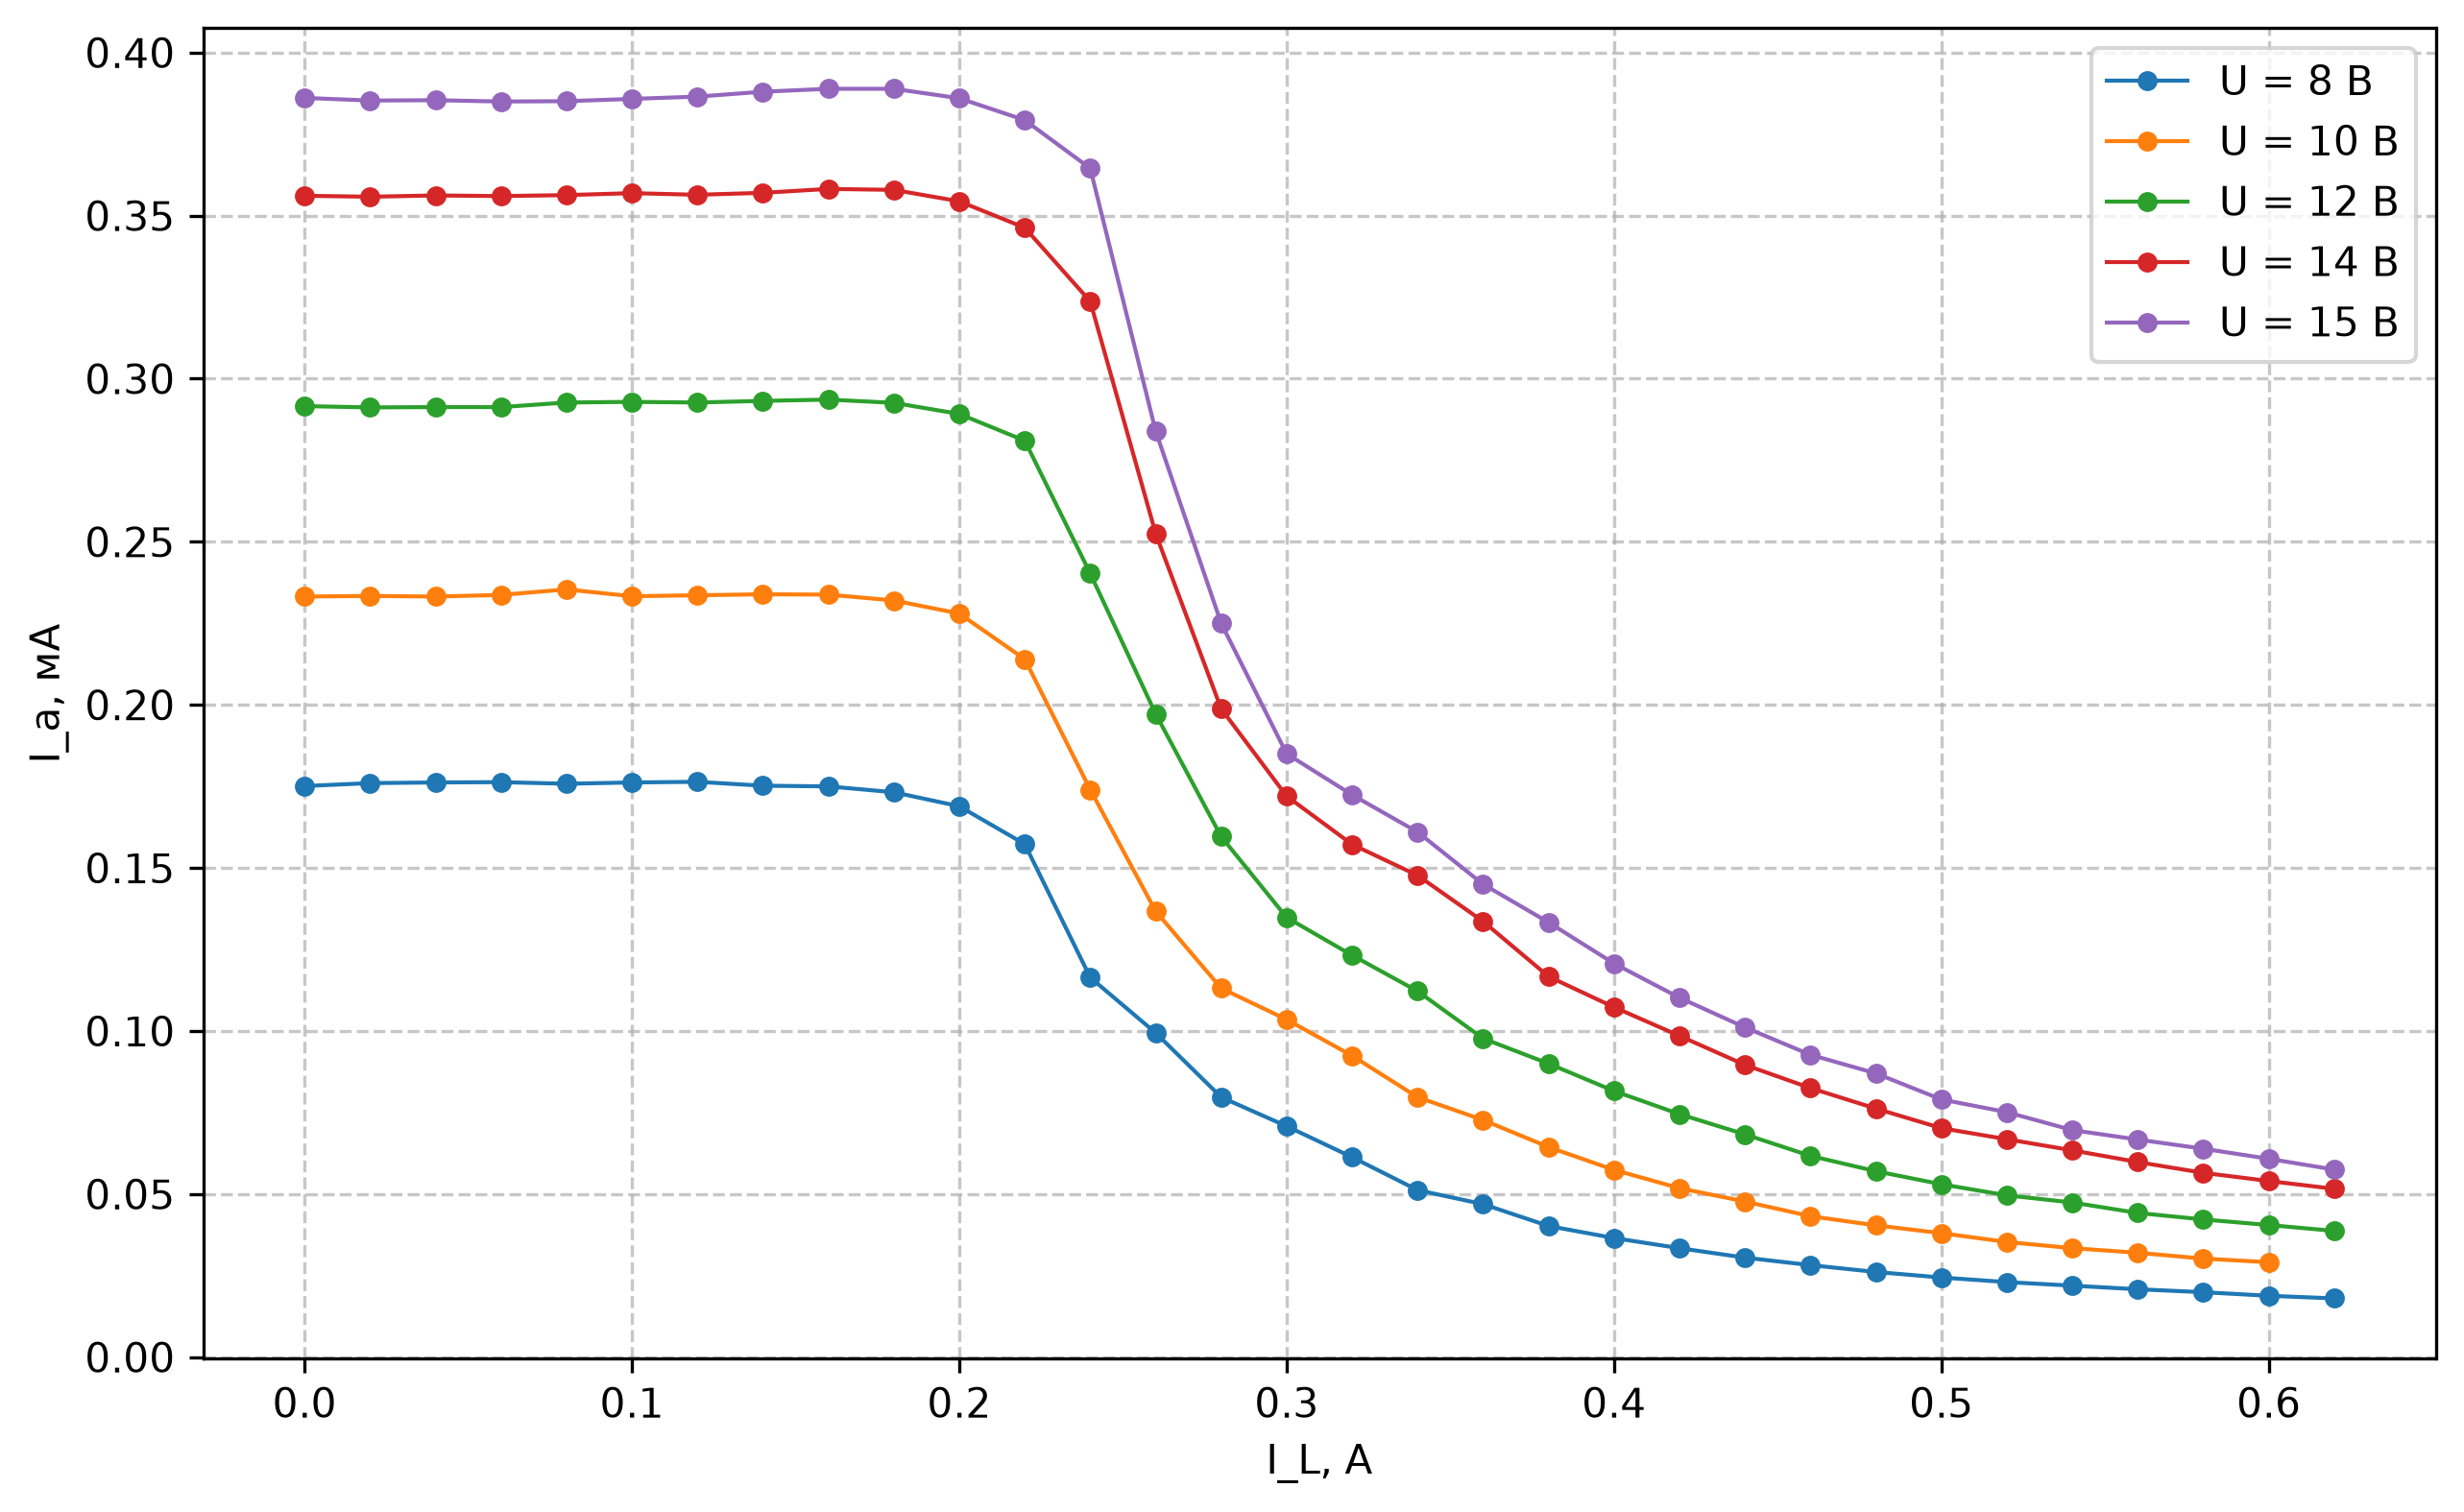
\includegraphics[width=0.95\textwidth]{fig1_combined.png}
    \caption{График зависимости анодного тока $I_a$ от тока соленоида $I_L$ для всех значений анодного напряжения}
    \label{fig:combined}
\end{figure}

\begin{figure}[H]
    \centering
    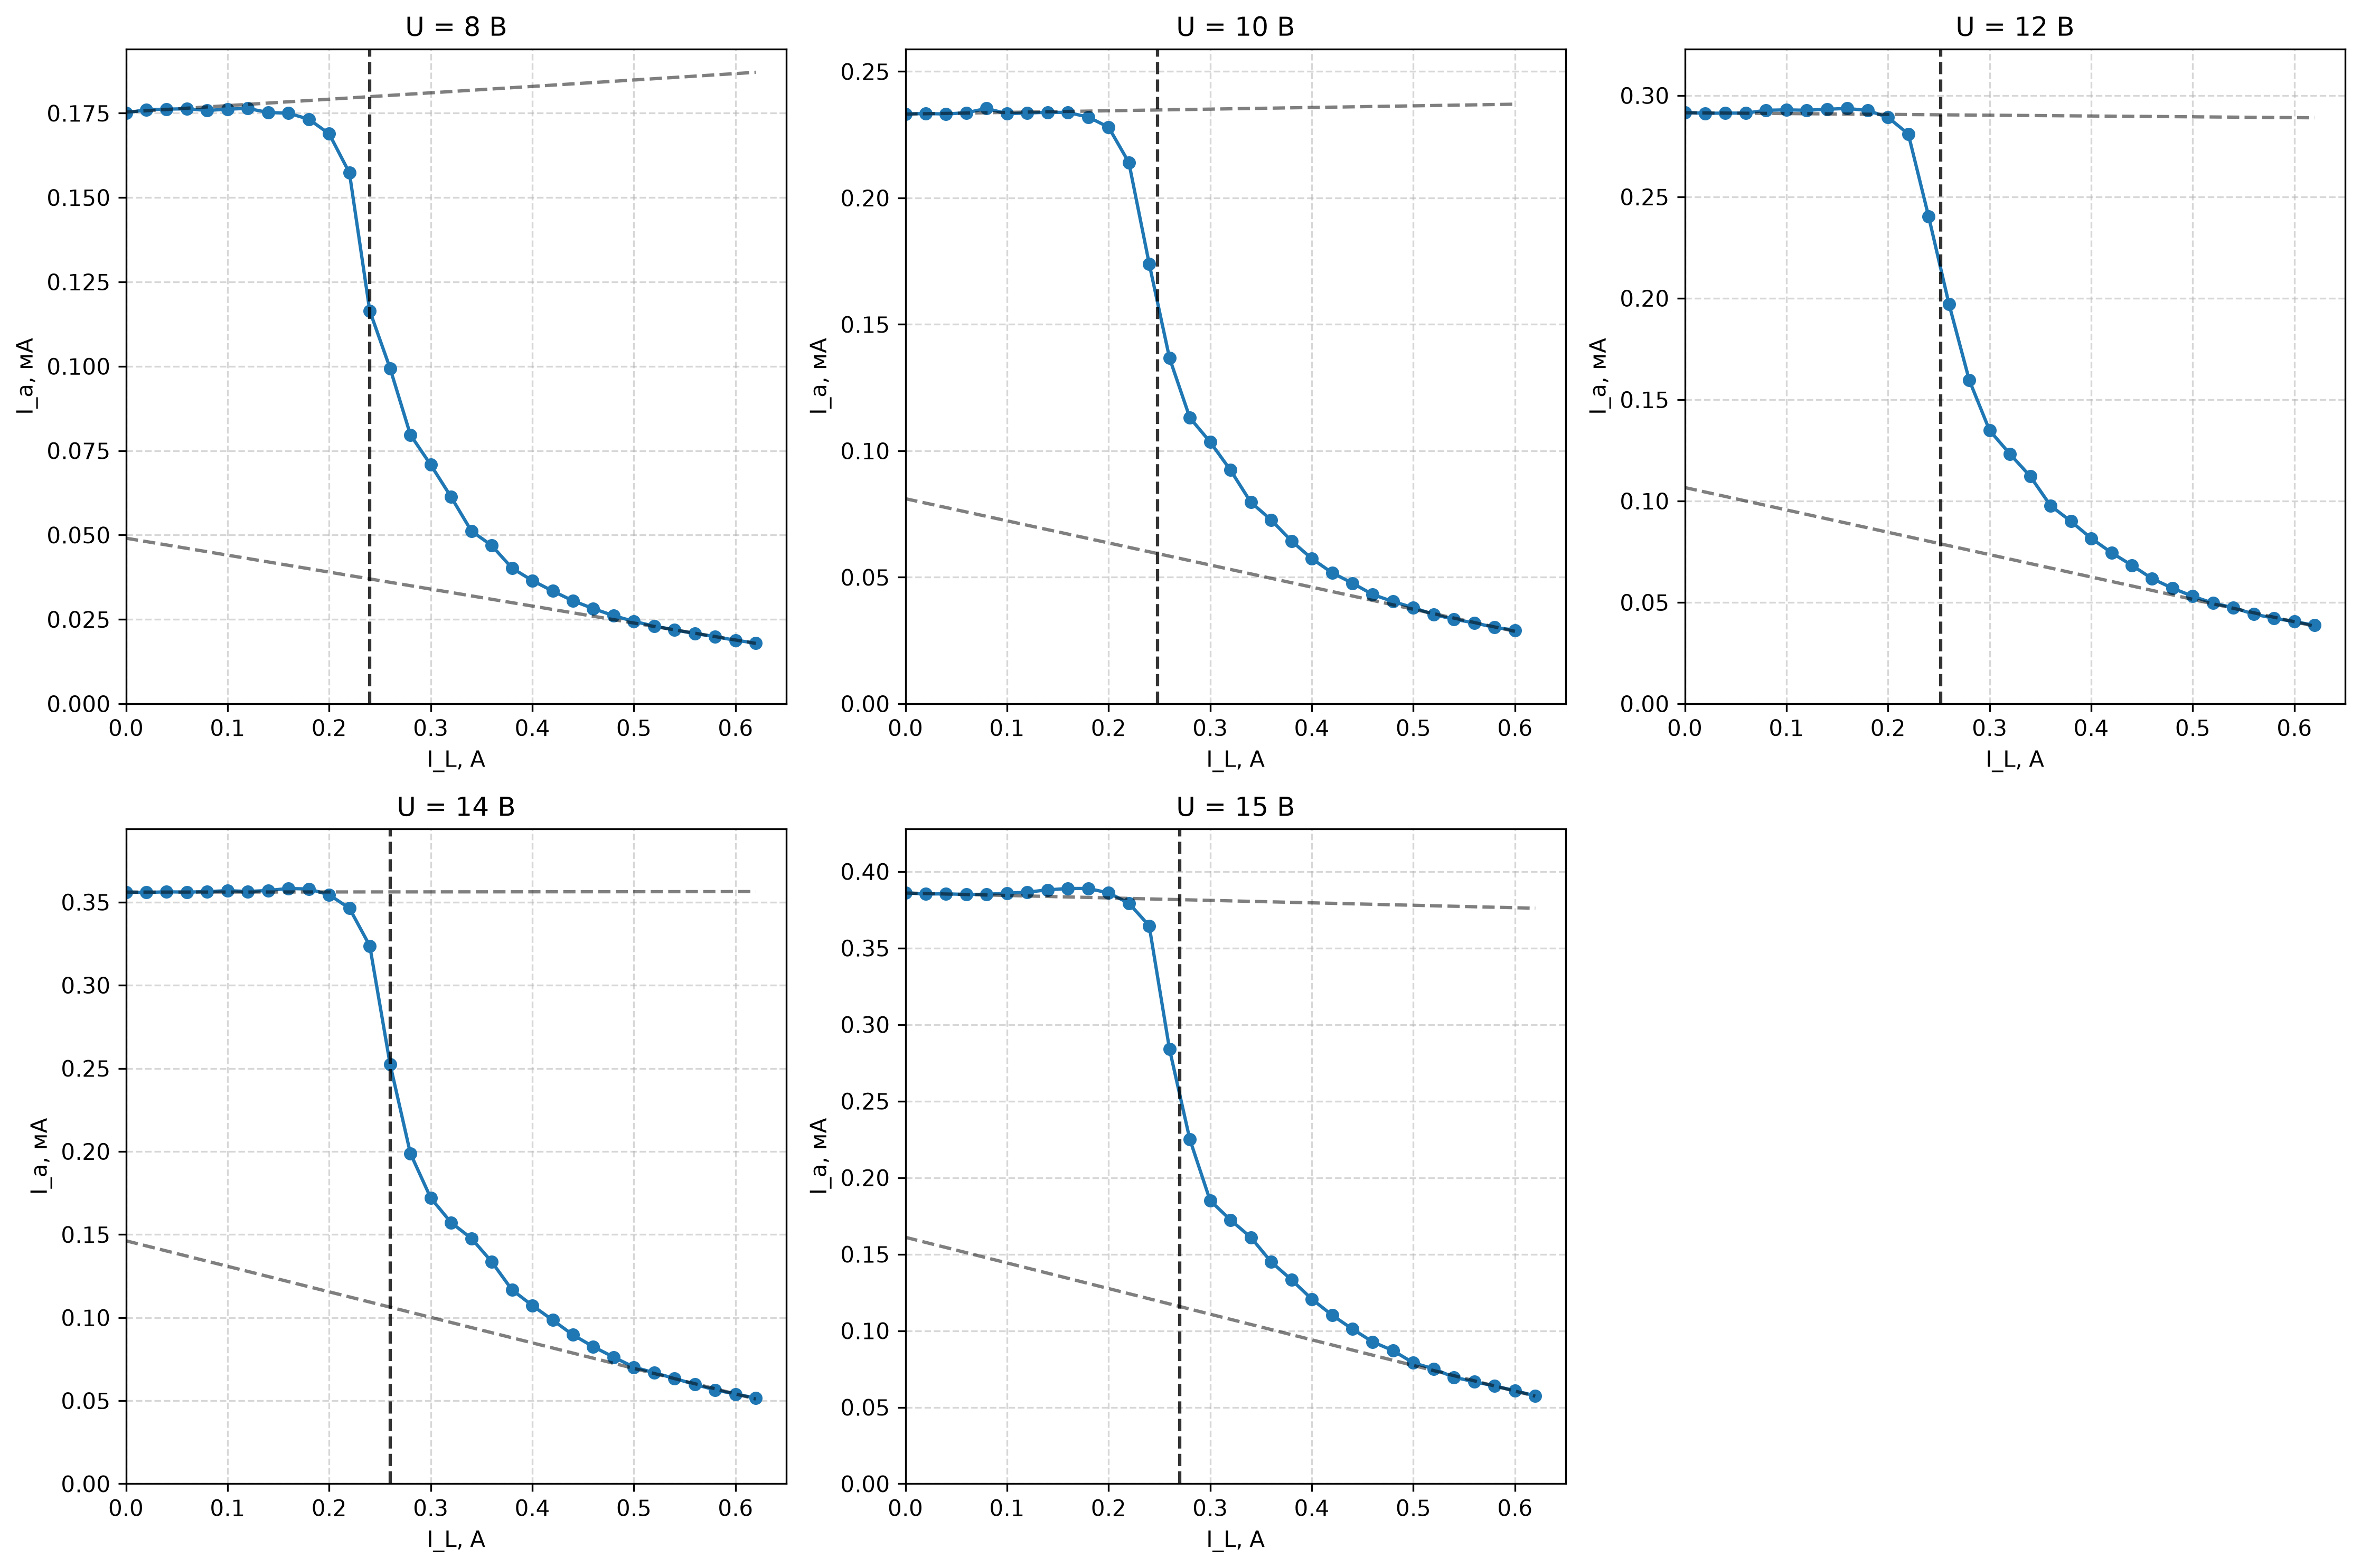
\includegraphics[width=0.95\textwidth]{fig2_geometric.png}
    \caption{Геометрическое нахождение критического тока $I_{L\text{кр}}$ (метод пересечения касательных)}
    \label{fig:geometric}
\end{figure}

\begin{figure}[H]
    \centering
    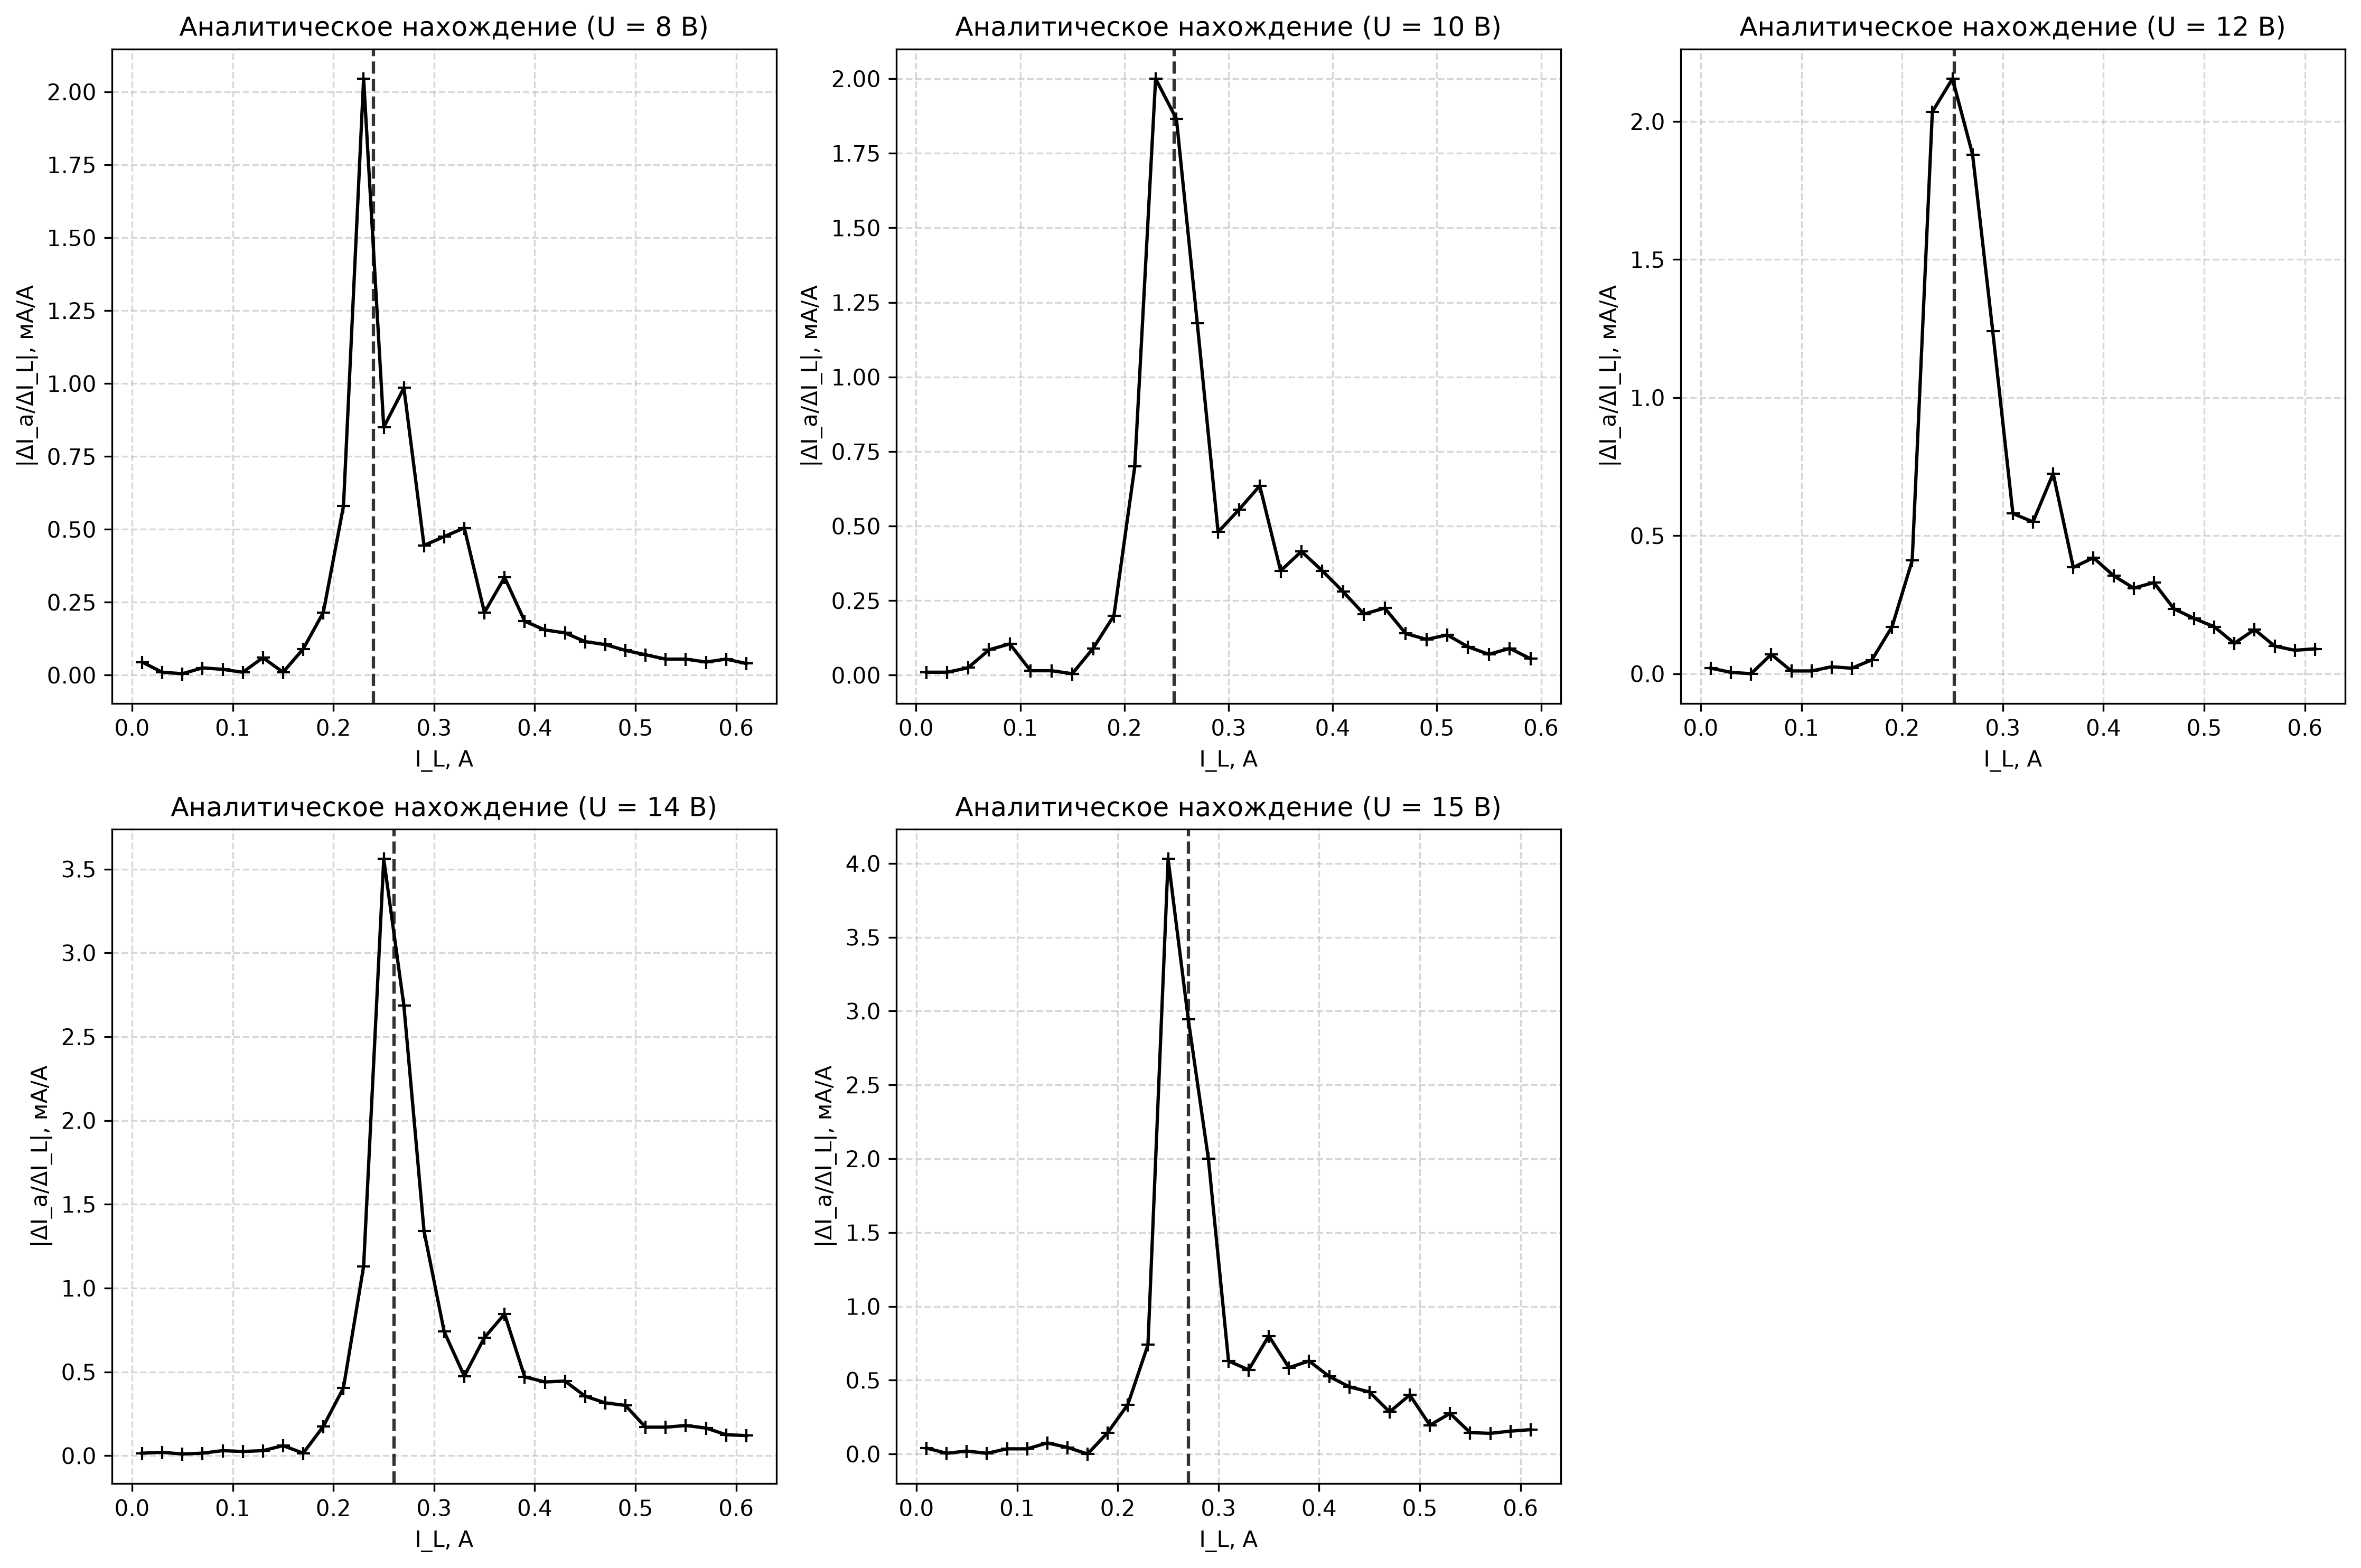
\includegraphics[width=0.95\textwidth]{fig3_derivative.png}
    \caption{Аналитическое нахождение критического тока $I_{L\text{кр}}$ (метод численного дифференцирования)}
    \label{fig:derivative}
\end{figure}

\begin{figure}[H]
    \centering
    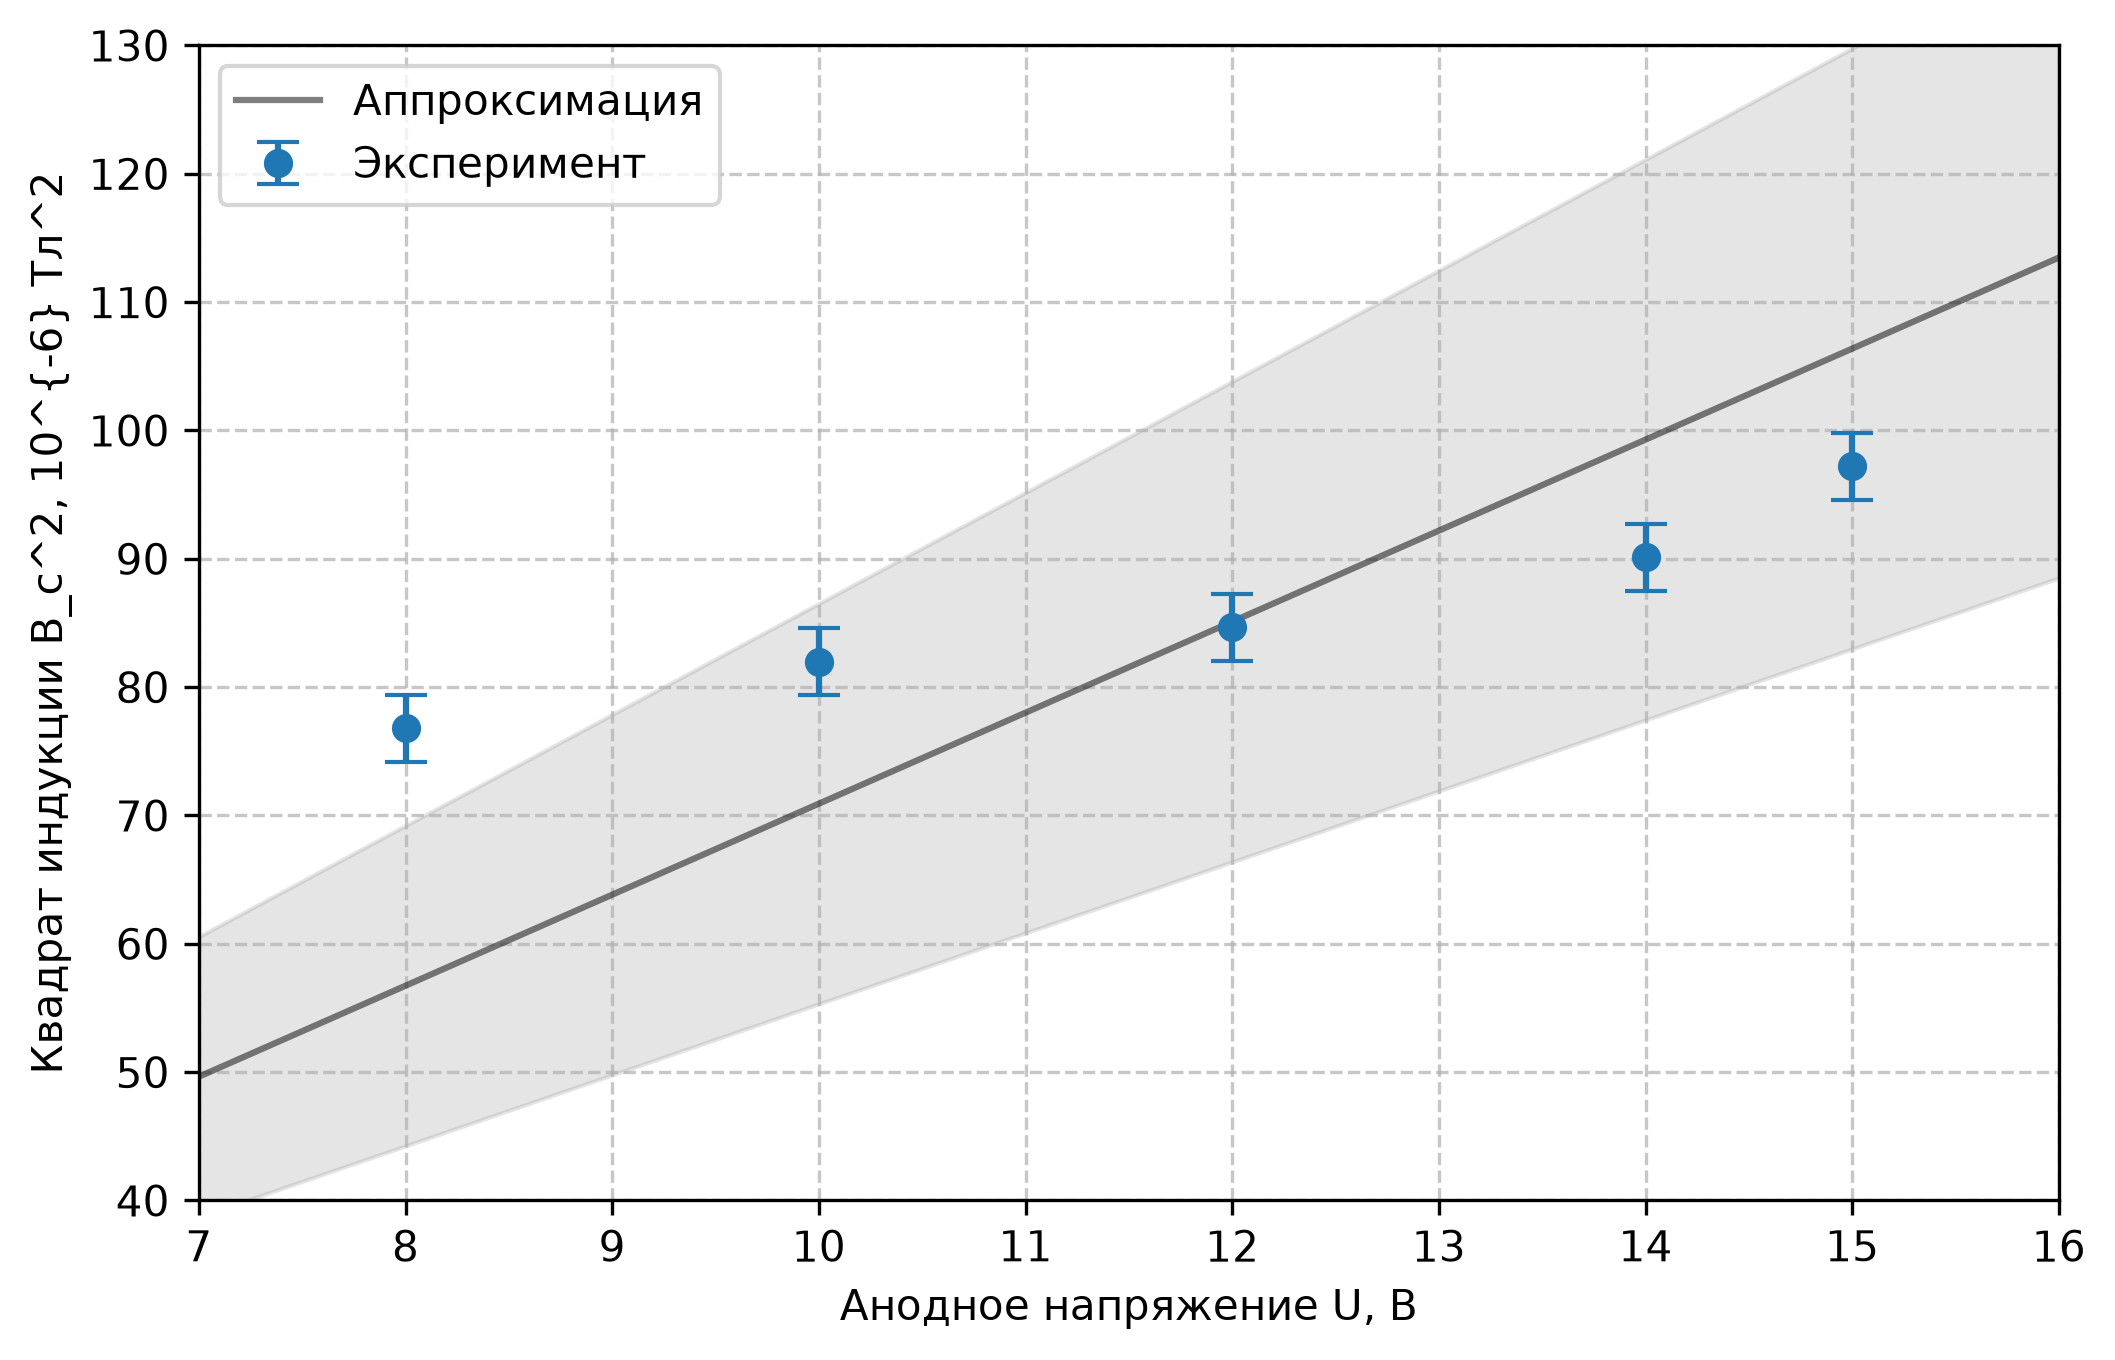
\includegraphics[width=0.8\textwidth]{fig4_regression.png}
    \caption{График зависимости квадрата индукции магнитного поля $B_c^2$ от анодного напряжения $U$}
    \label{fig:regression}
\end{figure}

\section*{\hspace{30pt}11. Окончательные результаты}

\hspace{15pt} Табличное значение удельного заряда электрона:
\begin{equation*}
    (e/m)_{\text{табл}} = 1.759 \cdot 10^{11} \text{ Кл/кг}
\end{equation*}

В ходе работы были получены следующие значения:

\begin{table}[H]
    \centering
    \begin{tabular}{|l|c|c|}
        \hline
        \multicolumn{1}{|c|}{Метод} & $e/m$, $10^{11}$ Кл/кг & Отклонение от табличного \\ \hline
        Среднее по отдельным измерениям & $1.20 \pm 0.24$ & $\sim 32\%$ \\ \hline
        График $B_c^2(U)$ & $1.25 \pm 0.28$ & $\sim 29\%$ \\ \hline
    \end{tabular}
\end{table}

\hspace{15pt} Значение, полученное графическим методом (из наклона прямой $B_c^2(U)$ методом наименьших квадратов), составило $(1.25 \pm 0.28) \cdot 10^{11}$ Кл/кг. Данное значение не согласуется с табличным в пределах рассчитанной случайной погрешности: табличное значение $1.759 \cdot 10^{11}$ Кл/кг лежит за пределами доверительного интервала $(0.97 \div 1.53) \cdot 10^{11}$ Кл/кг. Относительное отклонение составило около 29\%.

\hspace{15pt} Значение, полученное методом усреднения по пяти анодным напряжениям, составило $(1.20 \pm 0.24) \cdot 10^{11}$ Кл/кг. Оно также не согласуется с табличным: верхняя граница доверительного интервала ($1.44 \cdot 10^{11}$ Кл/кг) находится ниже истинного значения, а сама средняя величина занижена примерно на 32\%.

\section*{\hspace{30pt}12. Выводы и анализ результатов работы}

\hspace{15pt} В ходе работы методом магнетрона определен удельный заряд электрона. Отклонение полученных значений от табличного ($1.759 \cdot 10^{11}$ Кл/кг) составило $\sim 29\%$. Данное занижение закономерно для реальных учебных установок и вызвано следующими систематическими погрешностями, не учтенными в идеализированной теоретической модели:

\begin{enumerate}
    \item \textbf{Краевые эффекты:} магнитное поле на краях соленоида слабее расчетного. Для отсечения тока нужен больший $I_{L\text{кр}}$, что математически занижает итоговое $e/m$ (так как ток стоит в знаменателе).
    \item \textbf{Потери напряжения:} реальное напряжение $U$ между катодом и анодом ниже показаний вольтметра из-за падения на контактах.
    \item \textbf{Тепловая скорость:} электроны вылетают с нагретого катода с начальной скоростью, требуя более сильного магнитного поля для возврата.
    \item \textbf{Неидеальная геометрия:} несоосность электродов размывает границу сброса тока, внося погрешность в определение точного $I_{L\text{кр}}$.
\end{enumerate}

\hspace{15pt} Наиболее физически достоверным является результат, полученный из наклона прямой $B_c^2(U)$: $e/m = (1.25 \pm 0.28) \cdot 10^{11}$ Кл/кг. Разброс значений по отдельным напряжениям указывает на то, что модель идеального магнетрона лишь приближённо описывает реальную установку. Именно поэтому для повышения точности необходимо использовать графический метод усреднения (МНК), который позволяет сгладить флуктуации, нивелировать случайные и частично компенсировать систематические погрешности определения критического тока $I_{L\text{кр}}$. Эксперимент качественно подтвердил теорию метода магнетрона, а количественное отклонение полностью объясняется аппаратными особенностями установки.

\end{document}